\documentclass[a4paper,12pt]{article}
\usepackage{enumitem}
\usepackage{fancyhdr}
\usepackage{pgffor}
\usepackage{calc}
\usepackage{lastpage}
\usepackage{array}
\usepackage{tcolorbox}
\usepackage{amssymb}
\usepackage{marginnote}
\usepackage{float}
\usepackage{etoolbox}
\usepackage{xcolor}
\usepackage{longtable}
\usepackage[ngerman]{babel}
\usepackage[babel]{csquotes}
\usepackage[T1]{fontenc}
\usepackage{fontspec}
\usepackage[left=2.5cm,
    right=2.5cm,
    top=2.5cm,
    bottom=2.5cm]{geometry}

\MakeOuterQuote{"}

\newcounter{ctasks}
\setcounter{ctasks}{0}
\newcounter{cpoints}
\setcounter{cpoints}{0}
\newcounter{cepoints}
\setcounter{cepoints}{0}
\newcounter{ehtmppoints}
\setcounter{ehtmppoints}{0}
\newcounter{ehtpointsline}
\setcounter{ehtpointsline}{0}

\providetoggle{NOTDEBUG}
\settoggle{NOTDEBUG}{true}

\newcommand{\makestars}{\marginnote{$\bigstar$}}%\marginnote{\advance\leftskip-\directlua{tex.print(0.31*\theehtpointsline)}cm\foreach \n in {1,...,\theehtpointsline} {$\bigstar$}}}

\tcbset{sharp corners,colframe=black!50!black,colback=white}
\tcbuselibrary{most}
\newcommand{\eh}[1]{{\bigskip\setcounter{ehtmppoints}{0}\footnotesize\iftoggle{NOTDEBUG}{}{\noindent\begin{tcolorbox}[size=title,right=1cm,enhanced,breakable,title=Erwartungshorizont Aufgabe \thectasks]
\everypar={\setcounter{ehtpointsline}{0}}

\noindent#1

\bigskip\noindent \textbf{Erreichbare Punkte: \theehtmppoints}
\smallskip\noindent\end{tcolorbox}}\normalsize}}

%% POINT FROM =============================================================
% \newcommand{\point}[0]{\stepcounter{ehtmppoints}\stepcounter{ehtpointsline}\makestars}

\usepackage{amssymb}
\usepackage{marginnote}
\usepackage{xpatch}

\makeatletter
\newcommand*\@mn@lastypos{\relax}
\newcommand*\@mn@lastpage{\relax}
\newlength{\@mn@currmove}
\setlength{\@mn@currmove}{\z@}
\providecommand\@firstofthree[3]{#1}
\providecommand\@secondofthree[3]{#2}
%\providecommand\@thirdofthree[3]{#3}% Already defined in LaTeX from 1998/03/20
\@ifundefined{pdflastypos}{%
  \let\mn@lastypos\lastypos
}{%
  \let\mn@lastypos\pdflastypos
}
\xpatchcmd{\@mn@margintest}{%
  \protected@write\@auxout{\let\themn@abspage\relax}{%
    \string\newmarginnote{note.\@mn@thispage.\@mn@atthispage}{%
      {\themn@abspage}{\noexpand\number\mn@lastxpos sp}}%
  }%
}{% extend \newmarginnote by the y pos
  \protected@write\@auxout{\let\themn@abspage\relax}{%
    \string\newmarginnote{note.\@mn@thispage.\@mn@atthispage}{%
      {\themn@abspage}{\noexpand\number\mn@lastxpos sp}{\noexpand\number\mn@lastypos}}%
  }%
}{}{\undefined}
\xpatchcmd{\@mn@margintest}{%
  \edef\@mn@currxpos{\expandafter\@secondoftwo\@mn@currpage}%
}{% the x pos is now the second of three arguments and the third is the y pos
  \edef\@mn@currxpos{\expandafter\@secondofthree\@mn@currpage}%
  \edef\@mn@currypos{\expandafter\@thirdofthree\@mn@currpage}%
}{}{\undefined}
\xpatchcmd{\@mn@margintest}{%
  \edef\@mn@currpage{\expandafter\@firstoftwo\@mn@currpage}%
}{% the page number is now the first of three arguments
  \edef\@mn@currpage{\expandafter\@firstofthree\@mn@currpage}%
}{}{\undefined}
\xapptocmd{\@mn@margintest}{% now add the y pos testing and the offset
  \settowidth\@tempdima{\ensuremath{\bigstar}}%
  \ifx\@mn@lastpage\@mn@currpage
    \ifx\@mn@lastypos\@mn@currypos
      \global\advance\@mn@currmove\@tempdima
    \else
      \global\@mn@currmove\z@
    \fi
  \else
    \global\@mn@currmove\z@
  \fi
  \@ifundefined{@mn@currxpos}{}{%
    \edef\@mn@currxpos{\the\dimexpr \@mn@currxpos-\@mn@currmove\relax}%
  }%
  \global\let\@mn@lastpage\@mn@currpage
  \global\let\@mn@lastypos\@mn@currypos
}{}{\undefined}
\makeatother

\newcommand*{\point}{\stepcounter{ehtmppoints}\marginnote{\advance\leftskip-1.2cm\ensuremath{\bigstar}}}

%% POINT END ==============================================================

\usepackage[T1]{fontenc}
\usepackage{lmodern}
\rmfamily
\DeclareFontShape{T1}{lmr}{b}{sc}{<->ssub*cmr/bx/sc}{}
\DeclareFontShape{T1}{lmr}{bx}{sc}{<->ssub*cmr/bx/sc}{}

\newcommand{\task}[4]{\stepcounter{ctasks}\bigskip\noindent
\begin{tabular}{@{}p{14.2cm} >{\raggedleft\arraybackslash}p{1cm}@{}}
  \begin{minipage}[t]{14.2cm}
    \textbf{\textsc{#4 \thectasks}}. #1
  \end{minipage}
  & \textbf{#2P}
\end{tabular}
\nopagebreak
#3}

\newcommand{\newtask}[3]{\addtocounter{cpoints}{#2}\task{#1}{#2}{#3}{Aufgabe}}
\newcommand{\newextratask}[3]{\addtocounter{cepoints}{#2}\task{#1}{#2}{#3}{Zusatz}}

\newcommand{\printlines}[1]{\normalsize\iftoggle{NOTDEBUG}{\begin{flushleft}\begin{longtable}[t]{@{}p{15.8cm}@{}}\directlua{
        for i=0,#1 do
            tex.print("\\medskip \\\\ \\hline")
        end
    }\end{longtable}\end{flushleft}}{}\normalsize}
\newcommand{\thedate}{25. Januar 2023}

\title{Logik Beispielklausur}
\date{\thedate}

\pagestyle{fancy}
\fancyhf{}
\fancyhead[R]{Logik Beispielklausur}
\fancyhead[C]{\thepage{}{ / }\pageref{LastPage}}
\fancyhead[L]{\thedate}

\SetLabelAlign{center}{\hss\makebox[0pt]{#1}\hss}

\begin{document}
\begin{center}
    \Large Logik Beispielklausur
\end{center}

\newtask{Schreiben Sie hinter die folgenden Schemata die Buchstaben der Begriffe, ob das Schema \mbox{(A) \textit{allgemeingültig}}, \mbox{(E) \textit{erfüllbar}} und/oder \mbox{(W) \textit{widersprüchlich}} ist:}{4}{

\begin{enumerate}[label=\arabic*.,align=right]
    \item $(p \rightarrow p)$
    \item $(p \wedge \lnot p)$
    \item $((p \rightarrow q) \wedge p) \rightarrow q$
    \item $(p \downarrow q)$
\end{enumerate}

\eh{\begin{enumerate}[label=\arabic*.,align=right]
    \item \point (A), (E)
    \item \point (W)
    \item \point (A), (E)
    \item \point (E)
\end{enumerate}}
}

\newtask{Formalisieren Sie: \textit{"Wenn ich die Beispielklausur bestehe, schaffe ich Logik locker."}  Sei $p$ die hinreichende und $q$ die notwendige Bedingung in Ihrer Übersetzung. Kreuzen Sie an, welche der folgenden Schemata äquivalent zu Ihrer Formalisierung sind.}{5}{

\begin{enumerate}[align=center,label={$\bigcirc$}]
    % \item $\lnot p \lor p$
    \item $\lnot q \rightarrow \lnot p$
    \item $\lnot p \rightarrow q$
    \item $\lnot (p \wedge \lnot p)$
\end{enumerate}

\printlines{5}

\eh{Mögliche Formalisierung:

\bigskip\point p := "Ich bestehe die Beispielklausur."

q := "Ich schaffe Logik locker."

\point $p \rightarrow q$

\bigskip
Je nach Formalisierung entweder nichts oder ...

\begin{enumerate}[align=center,label={$\bigcirc$}]
    % \item[\otimes] \point $\lnot p \lor p$
    \item[\otimes] \point $\lnot q \rightarrow \lnot p$
    \item \point $\lnot p \rightarrow q$
    \item[\otimes] \point $\lnot (p \wedge \lnot p)$
\end{enumerate}}
}

\newtask{Beweisen Sie, dass \textit{"Unter allen Umständen ist es der Fall, dass ..."} ein logisches Partikel, aber keine Wahrheitsfunktion ist.}{7}{
\printlines{35}

\eh{\point \begin{tabular}{p{8cm}}
    Unter allen Umständen regnet es. \\ \hline
    Also regnet es auch, wenn die Sonne scheint.
\end{tabular}

\bigskip
\begin{tabular}{p{8cm}}
    Unter manchen Umständen regnet es. \\ \hline
    Also regnet es auch, wenn die Sonne scheint.
\end{tabular}

\bigskip\point Der erste Schluss ist gültig, der zweite nicht. Ersetzt man es durch \textit{"Unter manchen Umständen ist es der Fall, dass..."} wird der Schluss ungültig. \point Also ist es aufgr. der Def. LP. ein logisches Partikel.

\point Eine Wahrheitsfunktion ist es dann nicht, wenn zwei Sätze des gleichen Wahrheitswertes zusammen mit dem Satzteil zwei unterschiedliche Wahrheitswerte ergeben.

\point \textit{"Ich lebe." und "Menschen sind Menschen."} sind wahr. \point "Unter allen Umständen lebe ich." ist falsch, "Unter allen Umständen sind Menschen Menschen." ist wahr. \point Der Wahrheitswert hat sich geändert, aufgr. Def. WF. ist es keine WF.}
}

\newtask{Beweisen Sie mithilfe des Ersetzbarkeitsprinzips nach Leibniz "Nemo" und "Dora" nicht identisch sind.}{4}{
\printlines{15}

\eh{\point Zwei Wörter $\ulcorner\alpha\urcorner$ und $\ulcorner\beta\urcorner$ sind genau dann wahr, wenn es keinen wahren Satz gibt, in dem $\alpha$ und $\beta$ vertauscht werden können und sich der Wahrheitswert des Satzes ändert. \point Seien die Sätze \textit{"Nemo ist ein oranger Fisch."} und \textit{"Dora ist ein blauer Fisch."} wahr. \point Tauscht man "Dora" durch "Nemo" im zweiten Satz, wird daraus \textit{"Nemo ist ein blauer Fisch."}, ein falscher Satz. \point Der Wahrheitswert hat sich geändert, damit sind die beiden nicht identisch.}
}

\newtask{Beweisen Sie die Allgemeingültigkeit folgender Aussage: \textit{"Wenn es etwas buntes und schönes gibt, dann gibt es einiges schönes und mindestens auch eine bunte Sache."}}{8}{
\printlines{40}

\eh{\point "$F[1]$" := "$[1]$ ist bunt."

"$G[1]$" := "$[1]$ ist schön."

\bigskip \point Theorem: $\exists x (Fx \wedge Gx) \Rightarrow \exists x Fx \wedge \exists x Gx$

\bigskip Beweis:

\medskip \begin{tabular}{| c | c | c | c | c | c |}
\hline
\textbf{$\bigstar$} & \textbf{Nr.} & \textbf{Schema} & \textbf{B.} & \textbf{K.} \\ \hline
$\ast$ & 1 & $\exists x (Fx \wedge Gx)$ & & \point P \\ \hline
$\ast$ & 2 & $Fx' \wedge Gx'$ & 1 & \point $x'$ES \\ \hline
$\ast$ & 3 & $Fx'$ & 2 & AL \\ \hline
$\ast$ & 4 & $Gx'$ & 2 & AL \\ \hline
$\ast$ & 5 & $\exists x Fx$ & 3 & \point EG \\ \hline
$\ast$ & 6 & $\exists x Gx$ & 4 & EG \\ \hline
$\ast$ & 7 & $\exists x Fx \wedge \exists x Gx$ & 5,6 & AL \\ \hline
 & 8 & $\exists x (Fx \wedge Gx) \rightarrow \exists x Fx \wedge \exists x Gx$ & 1,7 & \point $\ast$Kd \\ \hline
\end{tabular}

\point \begin{enumerate}[label=\arabic*.]
    \item In der letzten Zeile und ihren Prämissen kommt keine geflaggte Variable vor.
    \item "$x'$" wurde nur einmal geflaggt.
    \item "$x'$" ist so eine Reihenfolge, da keine rechts oder links von ihr steht und sie daher nirgendwo frei vorkommen kann, wo eine rechts von ihr stehende gebunden ist.
\end{enumerate}

\point Die Ableitung ist fertig und aufgr. Def.$\Rightarrow$ ist das Theorem wahr, da in der letzten Zeile keine Sterne mehr vorkommen.}
}

\newtask{Füllen Sie die leeren Felder des logischen Quadrats korrekt aus!}{4}{

\begin{center}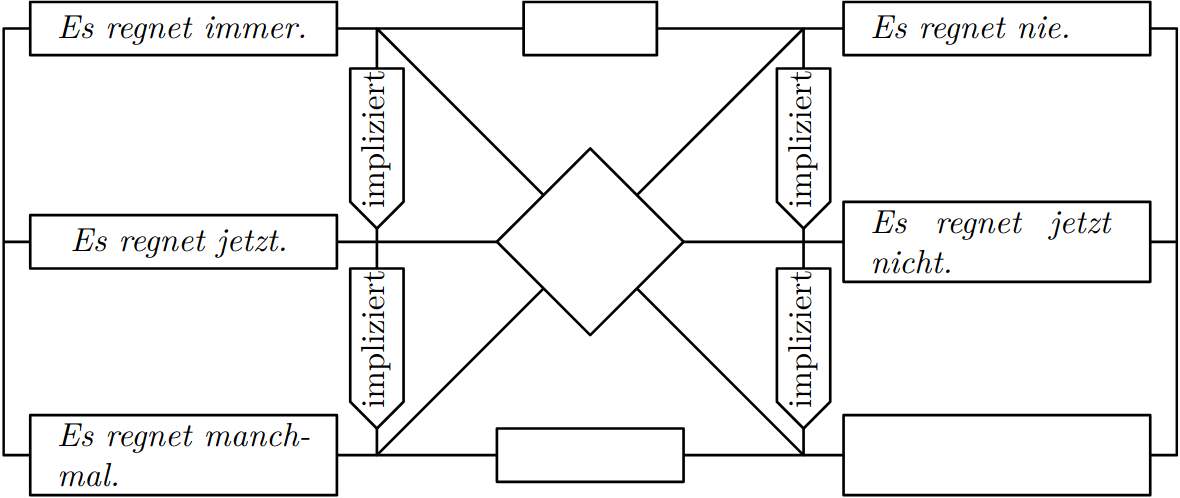
\includegraphics[width=14cm]{log_q_a.png}\end{center}

\eh{\begin{center}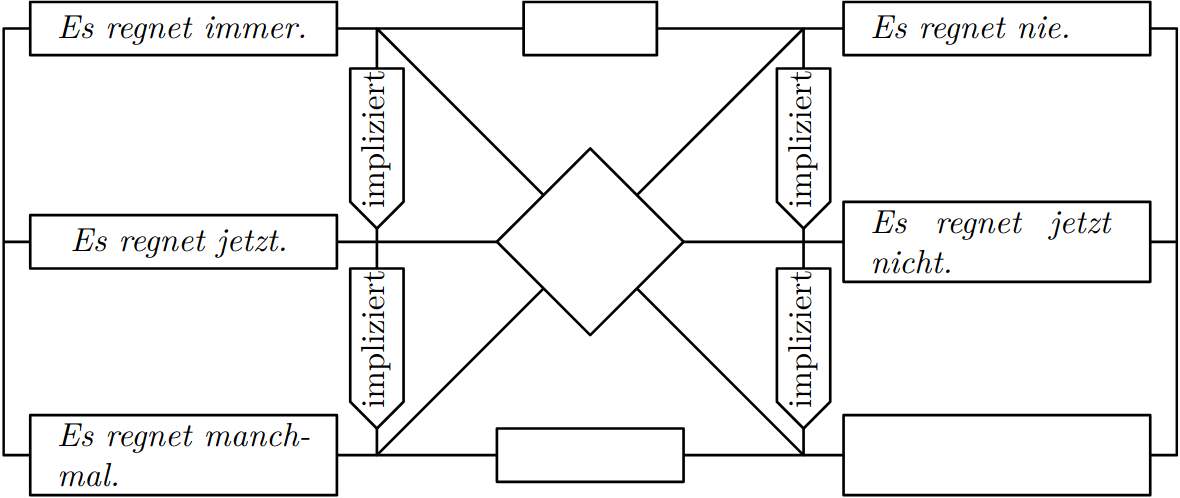
\includegraphics[width=13cm]{log_q_a.png}\end{center}

\begin{enumerate}[label=\arabic*.]
    \item \point konträr
    \item \point kontradiktorisch
    \item \point subkonträr
    \item \point Es regnet nicht immer.
\end{enumerate}}

\newextratask{Ist der folgende Schluss gültig? Entscheiden Sie und beweisen Sie Ihre Antwort!

\begin{quote}
  \textit{Wenn es regnet, dann ist die Stra{\ss}e nass. Es regnet oder es schneit, also ist die Stra{\ss}e nass, denn es schneit nicht.}
\end{quote}}{6}

\printlines{30}

\eh{\point "p" := "Es regnet."

"q" := "Es schneit."

"r" := "Die Stra{\ss}e ist nass."

\bigskip \point \begin{tabular}{c}
    $p \rightarrow r$ \\
    $p \lor q$ \\
    $\lnot q$ \\ \hline
    $r$
\end{tabular}

\medskip \begin{tabular}{| c | c | c | c | c | c | c |}
    \hline
    \textbf{$\bigstar$} & \textbf{$\bigstar$} & \textbf{$\bigstar$} & \textbf{Nr.} & \textbf{Schema} & \textbf{B.} & \textbf{K.} \\ \hline

    $\ast$ & & & 1 & $p \rightarrow r$ & & \point P \\ \hline
    & $\ast$ & & 2 & $p \lor q$ & & P \\ \hline
    & & $\ast$ & 3 & $\lnot q$ & & P \\ \hline
    & $\ast$ & $\ast$ & 4 & $p$ & 2,3 & \point AL \\ \hline
    $\ast$ & $\ast$ & $\ast$ & 5 & $r$ & 1,4 & \point AL \\ \hline
\end{tabular}

\bigskip \point Die Ableitung ist fertig, da keine Variable geflaggt wurde. Die Konklusion konnte aus den Prämissen abgeleitet werden, daher ist das Theorem wahr.}
}

\bigskip\noindent \textbf{\_\_\_ / \thecpoints{ + }\thecepoints{ }Punkten}. Zum Bestehen sind \textbf{\directlua{tex.print(math.floor(\thecpoints / 2))} Punkte} nötig.
\end{document}


